% Autor: Alfredo Sánchez Alberca (email:asalber@ceu.es)
% Charts that shows the purpose of Statistics
\begin{tikzpicture}[every label/.style={text=color1}]
\tikzstyle{node} = [align=center, node distance=1cm]; 
\tikzstyle{arrow} = [-latex, color2, line width=10pt];

\node (population) [label=90:Population] at (0,5) {\includegraphics[height=2cm]{img/introduction/population.pdf}}; 
\node (sample) [label=-90:Sample] at (0,0) {
\includegraphics[height=2cm]{img/introduction/sample.png}};
\node at (-0.5,2.6) [fill=color2,single arrow,shape border rotate=270,text=white, minimum width=1.2cm]{
\rotatebox{90}{Deduction}\phantom{}};
\node[node] at (-2,2.5) {From general\\ to particular};
\pause
\node at (0.5,2.4) [fill=color2,single arrow,shape border rotate=90,text=white, minimum width=1.2cm]{
\rotatebox{-90}{Induction}\phantom{}};
\node[node] at (2.1,2.5) {From particular\\ to general};
\end{tikzpicture} 